\documentclass{llncs} % , times

\usepackage{amssymb, amsmath, graphicx, ltxtable, longtable, tabularx, url, ragged2e, xspace, verbatim, fancybox,tikz}
\usepackage{scalefnt}
\usepackage{relsize}
\usepackage{paralist}
\usepackage{listings}

\usepackage{tikz} 


%\newcommand{\ggr}[1]{\textcolor{magenta}{comment Gerd: \textit{#1}}}
\newcommand{\ggr}[1]{} %\textcolor{magenta}{comment Gerd: \textit{#1}}}

\lstdefinestyle{code}{language=java,
        numbers=left,
        xleftmargin=1em,
        numberstyle=\tiny,
        showstringspaces=false,
        frame=single,
        basicstyle=\ttfamily\footnotesize,
        escapeinside={(*@}{@*)}
        }

\lstdefinestyle{rdfexample}{
	numbers=left,
	numberstyle=\tiny,
	%numbersep=0.1pt,
	xleftmargin=2em,
	showstringspaces=false,
	frame=leftline,
	basicstyle=\ttfamily\small,
        escapeinside={(*@}{@*)}
	}


\newcommand{\fs}{\textsf{F\#}\xspace}

\newcommand{\rr}[1]{\textbf{RR #1}}

%\newcommand{\nr}[1]{
%\begin{tikzpicture}[auto,node distance=1cm,thin] 
  %\tikzstyle{every node}=[shape=circle,draw=none, 
    %text=black] 
  %\node (1) {\texttt{NR #1}}; 
%\end{tikzpicture} }
%
%\newcommand{\tr}[1]{
%\begin{tikzpicture}[auto,node distance=1cm,thin] 
  %\tikzstyle{every node}=[shape=circle,draw=none, 
    %text=white,shading=ball] 
  %\node (1) {\texttt{TR #1}}; 
%\end{tikzpicture} }

\newcommand{\tr}[1]{\textbf{TR #1}}

%\newcommand{\rdfs}[3]{\textbf{#1}: $\frac{#2}{#3}$}
\newcommand{\rdfs}[3]{\textbf{#1}: $\frac{\texttt{#2}}{\texttt{#3}}$}

\pagenumbering{arabic}

\begin{document}
\title{Improving Programmability of Linked Data Sources}
 





\author{Gerd Groener\inst{1}, Kenji~Takeda\inst{2}, Don Syme\inst{2}, Ross McKinlay\inst{2}}
%\\ \textsf{groener@uni-koblenz.de}}

\institute{$^1$Institute for Web Science and Technologies, University of Koblenz-Landau, Germany \\
$^2$Microsoft Research Cambridge, UK}

%\institute{Institute for Web Science and Technologies\\
%University of Koblenz-Landau, Germany}

\maketitle

\begin{abstract}
Linked data sources benefit from the flexible data model of RDF that
can easily be extended and does not have a fixed schema.
While this representation facilitates the publication and distribution of
linked data on the Web, it complicates the integration and processing of
data from these sources in programming environments since programs usually
rely on types and schema information to internally organize their data.
In this paper, we present the design and implementation
of an RDF type bridge, which is a compile-time component and acts
as a programming interface for arbitrary external RDF data sources.
As a result, programmers can use the type bridge to write programs
that access and integrate external RDF data. By loading the bridge into
a program, the type bridge offers development support by an interactive exploration
of the data source and ensures strong typing of retrieved RDF data.
\end{abstract}


%Information in RDF data sources is given by a set of explicit statements.
%Additionally,  RDF inference consists of a set of rules to derive
%implicit information from RDF data. This inference relies on
%the data structure. When processing data in
%programs and workflows, further information like type statements
%can be derived based on the flow of the data. 
%In this paper, we present an integration of RDF inference in
%a data processing environment. 

%%%%%%%%%%%%%%%%%%%%%%%%%%%%%%%%%%%%%%%%%%
%\section{TODO: Proposals for title}
%
%Some ideas for the title:
%\begin{itemize}
	 %\item Towards a Data-oriented Type System in Programming Environments
%
   %\item A type Bridging technique for RDF data sources
	%
	  %\item Adapter Layer for Web data integration
%
   %\item Connected Programming
%\end{itemize}
%

%%%%%%%%%%%%%%%%%%%%%%%%%%%%%%%%%%%%%%%%%%%%%%%%%%%%%%%%%%%%%%%%%%%%%%%%%%%%%%%%%%
\section{Introduction}
\label{sec:intro}
%%%%%%%%%%%%%%%%%%%%%%%%%%%%%%%%%%%%%%%%%%%%%%%%%%%%%%%%%%%%%%%%%%%%%%%%%%%%%%%%%%%%%%

% we just want to improve the programmability in web applications for linked data

% problem
Publishing linked (open) data on the Web has become a success story during the last years.
RDF as the underlying representation formalism allows for flexible modeling of data such that
users are able to easily share, distribute and interconnect their own data all over the world.
Publishing and representing data on the Web is one side of the coin, but writing programs
and applications that access and smoothly integrate RDF data  is another, rather challenging issue.

One key problem is the  gap how data is processed in both areas.
RDF representation benefits from the flexible data model,
while software engineering environments and programming languages rely on powerful typing mechanisms
that guide programmers in their development by intelligent IDE support
and avoid run-time exceptions that might be caused by incompatible types.


% interesting
The integration of large external data into programs and programming environments
has already been investigated by dynamically typed programming languages.
However, as it is in the nature of these languages, without type support when writing program code.
Some initially approaches (cf.~\cite{Syme2012fsharp}) use adapter mechanism to integrate large data sources into statically
typed programs. They rely on a rigid and well-known schema of the data source.
Given such schema information, these approaches have led to good principles and powerful tooling to
allow for a smooth integration of external data.

Looking into linked data, the question arises whether
a smooth integration is even possible for RDF data sources.
In particular, we are faced with the following problems.
First, schema information might be partially unknown and even incomplete when data are accesses.
Instead, the structure among individuals, which is given in terms of properties between individuals,
might be used for a data access with respect to a certain structure.
Second, while the schema is rather fix, the underlying data tend to change rather often.
Thus, programs at run-time might incorporate such aspects.
Third, the sheer size of data sources (like DBpedia)  might lead to a large number of types
and accordingly to high type generation effort, while the program and system execution
only need a part of the generated types.
Thus, in an extreme case, this might even make the use of statically typed languages impossible.


%At a first glance, an alignment between schema information in RDF (RDFS) and types in programming languages
%is a rather straightforward means to allow for typing of data from RDF sources in program execution.
%This is even a rather fix ``bridge'' since the schema in RDF sources tend to change rarely,
%which is necessary for a stable type system.
%However, at program run-time, there is no straightforward way how to incorporate implicit,
%incomplete and steadily changing data from RDF sources within the execution of (statically) typed programs.
%
%%hard
%Integrating Web data sources into types programming environments is a rather challenging problem.
%First, data sources on the Web might be huge and are often connected to other sources and thus.
%
%(i) data change at run-time
%(ii) representations might be incomplete
%(iii) data-oriented representation vs. class centric modeling
%
%
%% related work
%Existing approaches: Type Provider
% Contribution

In this paper, we present an integration and type bridge from RDF data sources to
statically typed programming languages. We adopt the principles of \emph{type provider}
and define an adapter as a kind of programming interface
for statically typed programming languages to RDF data sources.
The resulting type bridge can be loaded into
programs as library in order to access an arbitrary external RDF data source,
which offers a SPARQL endpoint. The type bridge is used to (i)~retrieve data
from the RDF data source and (ii)~to statically type the retrieved data
and integrate these generated types into the type system of the host programming language.
The type bridge is implemented in \fs.

%%%%%%%%%%%%%%%%%%%%%%%%%%%%%%%%%%%%%%%%%%%%%%%%%%%%%%%%%%%%%%%%
%\section{Use Case and Application Context}
%\section{Context and Problem Description}
\section{What does Programming Linked Data Mean?}
\label{sec:context}
%%%%%%%%%%%%%%%%%%%%%%%%%%%%%%%%%%%%%%%%%%%%%%%%%%%%%%%%%%%%%%%%%%%%%%%%%%%%%%%%%%%%%%%%%%%%%%%%%%%%


The RDF  model is  a graph, which is constituted of a set of subject-predicate-object triples.
This graph covers both the schema in terms of classes and the data by individuals.
The usage of certain predicates like \texttt{rdf:type}, \texttt{rdfs:domain} and \texttt{rdfs:range}
and classes like \texttt{rdf:Class} indicate that certain entities in the graph are classes.
Thus, this is the only evidence for a schema.


\subsection{Exemplified Problem Description}

When writing programs and Web applications, programmers use programming languages and environments like IDEs
to write their code. 
Programming languages typically rely on some kind of schema or types
where types (or classes) serve as containers to manage data.
The organization of types in a so-called type system is an essential benefit of \emph{statically typed} languages where a powerful type system supports programmers during the program design and 
ensure type correctness in program execution. In particular, statically typed programming languages provide the following benefits:


\begin{enumerate}
	\item \textbf{Design Time Assistance:} The programming environment  supports programmers when writing code by
	 context-sensitive auto-completion, interactive type checking (so called red squigglies) and quick information display like mouse-hover
	and detailed documentation (e.g., by pressing the F1 button). All these interactive features help programmers in writing their code
	and give early feedback (at design time) about program correctness. 
	\item \textbf{Run-time Assistance:} When a statically program is compiled, type definitions and their usage in programs
	        are checked. Thus, at run-time, we can rely on a proper type system that offers features like type casts,
					 type checking and type inference. Run time errors and exceptions during program execution based on
					 incorrect type usage and type mismatch are already detected during design and compilation, and thus, might not
					cause errors at run-time. Types can be even used to optimize type interpretations.
					\ggr{I can't remember what the last sentence about optimize / drive interpretations mean.}
					
\end{enumerate}

While these benefits of statically typed programming languages are obvious,
the key question is how can such features be achieved when we integrate RDF data,
i.e., types in our type system refer to RDF classes and collections of individuals.
This means, that types are used in the usual programming manner, for instance RDF individuals
have all properties that are defined by the RDF classes. This is illustrated in the following example.
In each step, we see the corresponding requirement that has to be addressed by a type bridge.
We can distinguish between \emph{retrieval requirements (RR)} and \emph{typing requirements (TR)}.

Assume a developer is programming an application for a mobile phone to provide additional
data for movies like information about actors or genre. These additional data
are retrieved from RDF data sources like DBpedia\footnote{DBpedia: \url{http://dbpedia.org}} via a SPARQL endpoint,
e.g., as provided by DBpedia\footnote{DBpedia SPARQL Endpoint: \url{http://dbpedia.org/sparql}}.
These data should be included in the application on demand, i.e., only if needed
and they should be managed in the application in a typed fashion,
as described above.

\vspace{0.6em}
\noindent
\textbf{Step 1: Find a class.}
First of all, the programmer decides to use DBpedia as a data source since it is well connected to other
data sources. As a first step, the programmer has to look for a dedicated class for ``Actor'' in the data source.
For this purpose, the data source must be explored, e.g., by showing all RDF classes in a list
such that the developer can select the class of interest.

\rr{1}: Thus, we need means to explore a data source in terms of retrieving classes from RDF data sources.

\vspace{0.6em}
\noindent
\textbf{Step 2: Define a class / type for  an RDF class.}
Once, a class for an ``Actor'' is found, e.g., \texttt{http://dbpedia.org/ontology/Actor}, the programmer has
to define a corresponding type in the program.

\begin{lstlisting}[style=code, caption={Type Definition for RDF Class ``Movie''}, label={lst:movietype}]

// type definition for "Actor" 
type Actor = {
  id : URI
  rdfs:label : String 
}
\end{lstlisting}

\tr{1}: The problem that we have to solve here is to map the RDF class description into a type definition in the program code.
          This should be done automatically.

\vspace{0.6em}
\noindent
\textbf{Step 3: Define related types.}
Looking into the RDF class, we see that ``Actor'' is a subclass of ``Artist'' (\texttt{http://dbpedia.org/dbpedia-owl:Artist}).
Hence, if we want to reflect this, we need to define a type for class ``Artist'' too.

\begin{lstlisting}[style=code, caption={Type Definition for RDF Classes ``Actor'' and ``Artist''}, label={lst:worktype}]

// type definition for  "Artist" 
type Artist = {
  id : URI
  rdfs:label : String
}
// type definition for "Actor"  as subtype of "Artist"
type Actor = {
  inherit Artist
  id : URI
  rdfs:label : String
}
\end{lstlisting}


Obviously, besides the ``Artist'' class, other class might be created since the actor is related to them. This procedure might even continue since
these other classes like ``Artist'' can depend on further classes.

Given the sheer size of linked data sources (or even the linked data cloud), the key \emph{problem} is which classes need to be 
integrated in a program, i.e., for which RDF classes is a type definition necessary. Building types for all classes of a
data source is definitely not scalable, and even not needed since a particular application 
might only require a part of the classes.

\tr{2}: Thus, the question is whether it is possible to build types only \emph{on demand}.

\vspace{0.6em}
\noindent
\textbf{Step 4: Define individuals of classes.}
In our application, we want to manage concrete actors that can be derived from the data sources
as individuals of this class. Using a SPARQL query we can retrieve all individuals of class ``Actor''.
For instance, we get the individual \texttt{http://dbpedia.org/page/Bruce\_Lee} for the actor ``Bruce Lee''.
Accordingly, we can build an instance of movie.

\begin{lstlisting}[style=code, caption={Individual of  ``Actor'' }, label={lst:skyfall}]
let bl = Actor(`http://dbpedia.org/page/Bruce_Lee')
\end{lstlisting}

\tr{3}: Types are used to instantiate individuals. In this case, properties of the individuals are specified at the type level
          such that accessing these properties at the individual level conforms to the type characteristics.

\vspace{0.8em}
\noindent
\textbf{Step 5: Incorporate properties of individuals.}
It is in the nature of the flexible RDF model that properties can be defined for individuals 
without explicit definition of these properties for classes. For instance, the individual
``Bruce Lee'' has properties that are not stated as properties for the RDF class ``Actor''.

\tr{4} and \rr{2}: Properties of individuals have to be incorporated by types. From a programming language perspective,
this is a rather challenging issue since a type usually specifies properties, which can be even optional,
but in our case, the previously sketched type specification does not even know about additional properties,
and such a situation has to be avoided in typed programming languages.


%requires means for bridging between the data representation on the Web and 
%Assume data from Wikipedia should be incorporated in an application, e.g., a touristic company makes
%to use published and up-to-date data about cities, landscapes and prominent people that are associated with citites.
%To do this, the company decides to retrieve data from DBpedia and and completely include / integrate these
%data in their programs.
%When writing programs and Web applications that access these data and especially integrate them such that they
%In general, connecting and integrating information spaces in programming languages is an essential part on informaiton-rich programming.
%One of the most prominent source is DBpedia, where
%parts of Wikipedia data are represeted as RDF,  and access to these data is offered via SPARQL endpoints. 
%The linked data cloud is mainly accessibly by SPARQL requests, retrieving
%classes (schema information) and data.
%However, the integration of data into a statically typed programming language is more than querying a data source.



% figure system architecture


%%%%%%%%%%%%%%%%%%%%%%%%%%%%%%%%%%%%%%%%%%%%%%%%%%%%%%%%%%%%%%%%%%%%%%%%%%%%%
\subsection{Features of the Type Bridge}
%%%%%%%%%%%%%%%%%%%%%%%%%%%%%%%%%%%%%%%%%%%%%%%%%%%%%%%%%%%%%%%%%%%%%%%%

%Based on the mentioned retrieval and typing requirements,
%we discuss the key contribution of the presented type bridge
%and how the requirements are met.

%\subsection*{Programming Language and Environment}

The aim of the RDF type bridge (or RDF type adapter) is to create types for RDF classes that
are retrieved from linked data sources. 
In essence, the type bridge acts as a type provider in \fs that supports the integration of information sources
into \fs~\cite{Syme2012fsharp}. Type providers are means for data programming
in statically typed programming languages.
The general principle of type providers is 
to retrieve a well structured schema from (Web) data sources in order to build
the corresponding types at run-time.

In our case, we can not rely on a well structured schema, thus we have to
incorporate RDF modeling characteristics in order to integrate data into
a static type system. The closest related type bridge is the Freebase  
type provider that allows for the navigation within the graph-structure of
Freebase~\footnote{The Freebase Wiki about the Schema: \url{http://wiki.freebase.com/wiki/Schema}}.
The RDF type bridge contains the following additional aspects:

\vspace{0.6em}
\noindent
\textbf{Type Integration and Type Inference.}
When deriving RDF data from external data sources, the key problem is how to integrate
such types into the host programming schema. \\
\textbf{Feature:} Types are built based on the schema information that is obtained
from the RDF data source. The schema is derived by the 
usage of certain predicates like \texttt{rdf:type}, \texttt{rdfs:domain} and \texttt{rdfs:range}
and classes like \texttt{rdf:Class}.

\vspace{0.6em}
\noindent
\textbf{Scalable Type Definition on Demand.}
As data sources on the Web tend to be huge, it is not a promising idea to
build the types for all classes of a data source.
Obviously, types are only needed if particular applications need to access them.
\textbf{Feature:} On demand typing based on the current element. Types are created lazily.
To to this, we need an efficient management of the already created types in order
to avoid unnecessary type creating, which might be possible due to cycles in the RDF data. \\


%\vspace{0.6em}
%\noindent
%\textbf{Incorporate Data Changes.}
%It is obvious that RDF data change rather frequently, while the
%schema remains stable. Thus, it is meaningful to build types wrt.\ schema (at design time)
%and populate these types at run-time.\\
%\textbf{Contribution:} Types are built wrt.\ the schema (class definitions in RDF).
%Classes are populated by individuals at run-time.
%This implicitly also takes changes of the data (individuals) into account. \\


%\subsection*{Semantic Web and Linked Data}

\vspace{0.6em}
\noindent
\textbf{Derive fine-grained Schema from RDF Data.}
Hierarchies of classes and also properties in RDF data can be quite extensive.
Besides this, domain and range restrictions of properties that entities can be classes
in case this is not explicitly stated. \\
\textbf{Feature:} We incorporate RDF entailment regime, which is supported by SPARQL~1.1
in order to derive a fine-grained type system / schema.
While our type bridge is built to access and integrate RDF data into programs,
we also use Semantic Web technologies and built the data access upon
these existing means. In particular, we apply SPARQL queries, the SPARQL entailment regime, which
includes RDF(S) entailment, and we actually rely on best practices for publishing linked data.

\vspace{0.6em}
\noindent
\textbf{Typing of Classes base on Instance Properties.}
In RDF data sources, property specifications at the class level are often rare,
for instance in DBpedia classes have only three or four properties and these are actually
quite generic one, derived from super-classes. Instead, the most interesting way for navigating
is at the instance level. But, how can we cover properties if their corresponding class
in the programming language does not have this property. We can even not assume this property
for the class since the individuals do not necessarily share their properties. \\
\textbf{Feature:}  When defining a type for an RDF class, the type bridge offers two
possibilities. The basic principle is to add properties to the type definition that
are obtained as properties of the corresponding RDF class. As an addition,
properties that are only on the individual level are also specified at the class level.
This is done by sampling individuals of an RDF class and then choose the most common properties.
Both the sample size and the threshold for ``popular'' properties are given as parameters.




%%%%%%%%%%%%%%%%%%%%%%%%%%%%%%%%%%%%%%%%%%%%%%%%%%%%%%%%%%%%%%%%%%%%%%%%%%%%%%%%%%%%%%%%%%%%%%%%%%%%%%%%
\section{Foundations}

%%%%%%%%%%%%%%%%%%%%%%%%%%%%%%%%%%%%%%%%%%%%%%%%%%%%%%%%%%%%%%%%%%%%%%%%%%%%%%%%%%%%%%%%%%%%%%%%%%%

An RDF\footnote{RDF Primer: \url{http://www.w3.org/TR/rdf-primer}} data source contains at least one RDF graph, which is a set of RDF triples $(s, p, o)$
that consists of subject (s), predicate (p)  and object (o) (cf.~Def.~\ref{def:rdf}).

\begin{definition}[RDF Graph]
\label{def:rdf}
Let $U$ be a set of URIs, $L$  a set of literals and $B$ a set of blank nodes,
with $U \cap L \cap B = \emptyset$.
An RDF graph is defined as:
$G$ $=$ $\{ (s ,\ p , \ o) \in (U\cup B)\times U \times (U\cup L \cup B) \} $. 
\end{definition}


SPARQL\footnote{SPARQL 1.1 Query Language: \url{http://www.w3.org/TR/sparql11-query}} 
is a query language for RDF graphs with  \textsf{select}, \textsf{from} and \textsf{where} clauses.
Like an RDF graph, the graph pattern of the \textsf{where} clause consists of RDF triples, in which
variables are allowed as subjects, predicates and objects of triples.
The result of a query is a binding of the variables in the \textsf{select} clause,
while the binding is determined by matching of triples from the \textsf{where} clause
to triples in the RDF graph $G$.

In SPARQL 1.1, which we are referring to in this paper, the graph matching principle between triples in the query and the data source
is extended by entailment relations, as defined by the SPARQL entailment regimes\footnote{SPARQL 1.1 Entailment Regimes:
\url{http://www.w3.org/TR/sparql11-entailment}}. Among others, the entailment regimes contain RDF and RDFS entailment rules
Thus, triple matching is extended to triples that can be derived from an RDF graph $G$. Formally, we denote
this extended set of triples, which can be derived by RDF(S) entailment, as Materialized Graph (cf.~Def.~\ref{def:mat}.A).
(The symbol $\models_{\mathcal{T}}$ denotes RDF(S) entailment.)

We use a distinction between classes (schema) and data in the RDF graph.
We refer an entity $C$ (subject or predicate in a triple) as a class (or RDF class).
This is described in Def.~\ref{def:mat}.B.
 

\begin{definition}[Materialized RDF Graph and RDF Classes]
\label{def:mat}
Let $\mathrm{G}$ be an RDF graph.
\begin{itemize}
	\item[A.]  A materialized graph $\hat{G}$ is defined as follows:

$\hat{G}$ $=$ $\{ (s ,\ p , \ o) \in (U\cup B)\times U \times (U\cup L \cup B) \ | \ G \models_{\mathcal{T}} (s, \ p, \ o) \}  $. 

\item[B.] $C$ is referred to as a class (or RDF class) if at least one of the following conditions hold:
(i) there is a type statement  (s rdf:type C) $\in \hat{G}$,
 (ii) there is a domain restriction (s rdfs:domain C) $\in \hat{G}$ or 
(iii) there is a range restriction (s rdfs:range C) $\in \hat{G}$ and C is not a data-type.
\end{itemize}
\end{definition}



%These rules derive implicit relations between classes, individuals and classes for individuals (\textsf{instanceOf} relation) based
%on explicit stated relations and domain and range restrictions of properties.

Types classify the kinds of individuals (or objects) that are manipulated in a program or application.
A type system is a syntactic technique to classify statements in order to avoid unintended program behavior.
We consider a type system as specified in Def.~\ref{def:type}. 

\begin{definition}[Type System]
\label{def:type}
Let $U$ be a set of URIs, $L$  a set of literals.
A type system consists of a domain $\Gamma$,
a set of entities M $(M \subseteq \mathcal{P}(U \cup L))$ and type expressions (or types for short) $\tau$.
The statement $\Gamma \vdash M: \tau$ means that entity $M$ has type $\tau$ in a domain / environment $\Gamma$.
\end{definition}




%%%%%%%%%%%%%%%%%%%%%%%%%%%%%%%%%%%%%%%%%%%%%%%%%%%%%%%%%%%%%%%%%%%%%%%%%%%%%%
\section{A Type Bridge for RDF}  
\label{sec:design}
%%%%%%%%%%%%%%%%%%%%%%%%%%%%%%%%%%%%%%%%%%%%%%%%%%%%%%%%%%%%%%%%%%%%%%%%%%%%%%



Our goal ist to build an integration bridge for arbitrary RDF data sources with a SPARQL endpoint
in order to access and integrated RDF data into a statically typed program on demand.
When using these bridge, it should not be part of the actual developed application,
instead it is just used as a library. In the following, we will see some technical details how
the bridge is developed.

\subsection{Features of the Type Bridge}
  
According to Sect.~\ref{sec:context}, we aim at achieving two groups of requirements:
retrieval requirements (RR) and typing requirements (TR). Retrieval is needed since  an RDF graph does not explicitly 
distinguish between schema and data, as in relational databases. Thus, the retieval is
used to find those elements in the graph that should be integrated as types and their corresonding data (individuals) in a program.
Aspects of the integration into the programming type system are reflected by the typing requirements (TR).

In order to meet these requirements, the type bridge has to provide the following functionality.
First, the exploration of an RDF graph must be supported. Thus, we need some kind of data handler
to be able to hook into the RDF source. Second, we have to use the data handler to explore the data source by
following the properties from one entity to the next one. This must be provoded for RDF classes and individuals.
Properties also include type statements, and therefore,
we can also follow relations between classes and individuals.
Third, the retrieval of the currently explored entity and its properties must be supported.
Fourth, The definition of a static type must be able. Thus also all properties of
the type must be defined.

The type bridge, its features and its context of use is illustrated in Fig.~\ref{fig:context}.
The type bridge consists of a connector and a type  generation descripition. The bridge uses
SPARQL to connect to an RDF data source. The program, which uses the type bridge, has to use
a data handler to get data from the data source and to finally build the types for retrieved data.
\begin{figure}
	\centering
		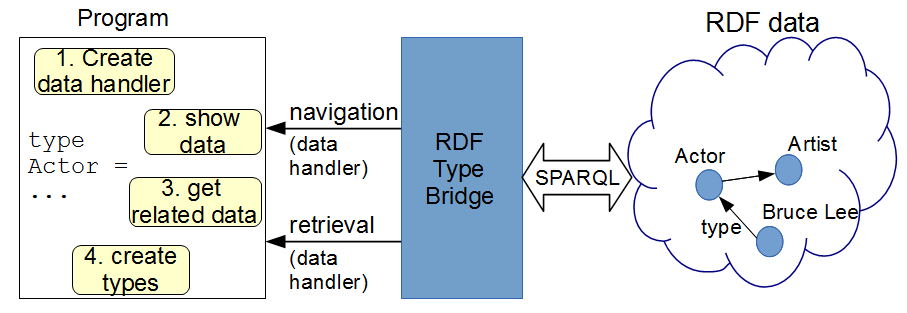
\includegraphics[width=0.98\linewidth]{./figs/context.png}
	\caption{Functionality and Context of the Type Bridge}
	\label{fig:context}
\end{figure}



\subsection{Type Definitions}

Our type bridge is a compile time component. It has static parameters like
the address (URI) of the SPARQL endpoint.
The type bridge consists of two components: (i)~the data source \emph{connector} and (ii)~the
\emph{type generation description}. The latter one is a kind of compile-time meta-programming construct.
In the following, we consider both components in detail.

The \emph{connector} establishes a connection to the SPARQL endpoint. It serves as a mediator
between the type generation descrition and the external data source.
The connector gets as an argument the URI of the SPARQL enpoint
in order to establish a connection to the SPARQL endpoint.

All data are obatined from the data source by SPARQL queries.
Thus, the connector consists of functions that are used by the type generation description
to navigate in the data source and to retrieve data from the source.
Internally, these functions encode SPARQL queries in order to implement both tasks the navigation and the retrieval.

Functions of the connector are used to retrieve (i)~all classes of the source,
(ii)~individuals of a certain class, (iii)~properties of a class (i.e., the objects of
triples in which the class is the subject and the property the predicate),
(iv)~properties of an individual and (v)~the classes of an individual.
The notion of a class in the RDF data referes to the specification of Def.~\ref{def:mat}.


%
%
%After a successful connection to the SPARQL endpoint, we get the following 
%artefacts for data access and connection:
%
%\begin{enumerate}
	%\item The \emph{signature} of the data source, which is given by classes and properties in 
	  %the data source, is retrieved.  \ggr{not really retrieved --- can be retrieved}
	%\item The \emph{type creating} on  demand.
%\end{enumerate}	



The key part of the type bridge is the \emph{type generation description} that
defines how types with their parameters, properties and methods are built when the bridge is used.
In essence, the type bridge is a model that specifies the type import into a language.
This type import is specified by a set of rules. 

Before we discuss these rules, we present one basic construct, the data handler or data context provider,
 of the type bridge that is  used by programs to work with the type bridge.
The type bridge itself specifies one base type, let's call it \texttt{rootType}. This type
is created whenever a program uses (and therefore instantiates) the type bridge.
The corresponding specification is shown in Listing~\ref{lst:root}. The argument ns denotes the namespace.

The \texttt{rootType} has one method (line 3, 4 in Listing~\ref{lst:root}) that
returns the data handler, which is later used in the program environment to handle the
connection to the type bridge. The \texttt{InvokeCode} specifies that when the method \texttt{getDataHandler}
is called, the \texttt{Connector}, according to the above description, is intialized. The argument is the URI
of a SPARQL endpoint (e.g., the endpoint URI of DBpedia). 

\begin{lstlisting}[style=code, caption={\textbf{Basic Rule:} For the generation of a root type with data handler}, label={lst:root}]
let rootType = ProvidedTypeDefinition(ns, rootTypeName,
   baseType=Some typeof<obj>)
let m = ProvidedMethod("GetDataContext", [], 
    InvokeCode = (fun _ -> <@@ Connector(sourceUrl) @@>))       
\end{lstlisting}

In the following, we describe  rules for building type definitions.
The first step is the definition of the type for RDF classes, which can be used in programs
to define types for RDF classes from the data source.
The type definition requires at least the name of the type and its erasure, i.e., the type this type can be erased to.

Let C be the class that is retrieved by a SPARQL query. The type generation description in \fs
is as follows:

\begin{lstlisting}[style=code, caption={\textbf{Type Rule:} Type Generation Description for RDF Class C}, label={lst:providedClass}]
t = ProvidedTypeDefinition(cname, baseType=Some typeof<obj>)
\end{lstlisting}

In Listing~\ref{lst:providedClass}, \texttt{cname} denotes the name of class $C$, e.g., the string of the URI of $C$.
The \texttt{baseType} gives the erased type, a``super-type'' from which the generated type  inherits.
For instance, an RDF class can just be erased to an \fs object type. If a type should have other features
like being iterable, the type can be erased to sequence or list and thus, this type can serve as a collection
element and iteration features on its elements will part of the type characteristics.

This type rule would be used if a programmer specifies a description for an RDF class.
This description, which is a compile-time meta-programming constuct, is
used to build the concrete RDF class, e.g., the ``Actor'' class in our example.


Types can have properties. Accordingly, if a type will be created, the corresponding properties
have to be created too. These properties are obtained from the RDF data source and should
be directly reflected in the source code that will specify the corresponding type.
Accordingly, the type generation description describes how to obtain properties and to
generate the properties of these types.

\begin{lstlisting}[style=code, caption={\textbf{Property Rule:} Add Property for Class C}, label={lst:providedProp}]
 let p = ProvidedProperty(pname, typeof<string>, 
    GetterCode = (fun args -> 
		     <@@(%%(args.[0]):obj) :?> string  @@>))
  // add this property (delayed)
 t.AddMemberDelayed(p)
 \end{lstlisting}

In Listing~\ref{lst:providedProp}, \texttt{pname} denotes the name of the property (e.g., the URI), \texttt{typeof} gives the
super-type (string in this case) and \texttt{GetterCode} is a so-called quotation that specifies the result of a property selection at run-time.
In this simple case, the string representation of the property itself is the meaning of the property. Such a provided property
is created for each property of the RDF class $C$.
In the second line, the peroperty is lazily ``added'' to the type. Here, type symbol $t$ referes to the
type of RDF class $C$. Note, the added properties depend on the concrete generated type 
when the bridge is used. For instance, if a type for RDF class ``Actor'' is created (according to the rule in Listing~\ref{lst:providedClass}),
the properties (predicates in the RDF graph) of ``Actor'' are generated and added (according to the property rule in Listing~\ref{lst:providedProp}).

In the next rule, we treat individuals. They can be added to their corresponding classes.
The according type generation description  is shown in Listing~\ref{lst:providedIndColl}.
For this, a new type would be created with the name of the class (denoted by \texttt{cname}) and the
suffix ``Individuals''. This type is added to t. In this collection, all individuals are contained.
We can see that the erased type (base type) of the individuals peroperty is a sequence (seq).

\begin{lstlisting}[style=code, caption={\textbf{Individual Rule:} Add Individuals (set / collection) to Class C}, label={lst:providedIndColl}]
let individuals = 
  ProvidedTypeDefinition(cname+"Individuals",
	   Some typeof<seq<obj>>)
// add these individuals
individuals.AddMembersDelayed()
//  add indiviual collection to type 
t.AddMemberDelayed(indiviuals)
 \end{lstlisting}




\subsection{Additional Constructs}

Types are created when a certain entity is retrieved from the graph, while this entity (e.g., a class) is reached
by navigating along the graph. Thus, we can also have some cycles in the exploitation. In order to achieve scalability in
statically typed languages, we have to ensure that a type for an entity is only created once.
To do this, we manage types in dictionaries i(hash maps) to ensure that types are unique.

Another technique that we apply is the sampling of properties. According to requirements \tr{4} and \rr{2},  a typed access on individuals
suffers from the problem that the type definition (based on the RDF class) to not necessarily reflect all property statements
of the individuals. To remedy this, we apply a sampling technique whenever a class type is created.
A static parameter of the type bridge gives the number of sampled individuals. The properties of these individuals
are added as optional properties to the corresponding types. Further parameters allow to specify
how often a property must appear in order to be added.
The rule for creating a property (Property Rule), as shown in Listing~\ref{lst:providedProp},
is the same, but it considers also these additional properties that are  sampled from
the individuals.
	
%%%%%%%%%%%%%%%%%%%%%%%%%%%%%%%%%%%%%%%%%%%%%%%%%%%%%%%%%%%%%%%%%%%%%
\section{Linked Data Programming --- the Type Bridge in-use}
\label{sec:usage}
%%%%%%%%%%%%%%%%%%%%%%%%%%%%%%%%%%%%%%%%%%%%%%%%%%%%%%%%%%%%%%%%%%%%

The type bridge, as presented in Sect.~\ref{sec:design}, can be applied for arbitrary RDF data sources.
The contribution of the type bridge is twofold. First, when writing a program, e.g., an application for a mobile phone (cf.~Sect.~\ref{sec:context}),
the programmer gets the full support from the underlying static type system. This includes programming environment
or IDE support like auto-completion, interactive type checking and error highlighting.
Second, when the application is used at run-time, these generated types behaves as basic .NET types in \fs.

Consider again the program development from the original example in Sect.~\ref{sec:design}.
When developing a progam by using the RDF type bridge, the libarary of the bridge (dll-file) must
be loaded and then a data handler is created, which invokes the connector component to
establish a connection. Afterwards, the data handler
serves as an object in the program to retrieve and organize the retrieved data during the development.

\subsection{Integrated Data Retrieval}
\label{sec:usage:retrieval}

The retrieval of RDF data is completely integrated in the IDE of the programming language,
i.e., Visual Studio\footnote{Visual Studio: \url{http://www.microsoft.com/germany/visualstudio/}}
or MonoDevelop\footnote{MonoDevelop IDE: \url{http://monodevelop.com/}} (for Linux systems).
Thus, a developer can explore an external RDF data source and retrieve data from this source
within the development environment  by using the data handler. Accessing the data handler is done by using  the usual dot-operator.
The data handler is obtained by calling the \texttt{GetDataContext()} method 
as outlined in Fig.~\ref{fig:getdc}.

%\begin{lstlisting}[style=code, caption={Initialize data handler}, label={lst:useTP1}]
%let dc = RdfTypeProvider<"http://dbpedia.org/sparql">.getDataHandler()
%\end{lstlisting}


\begin{figure}[h]
\centering
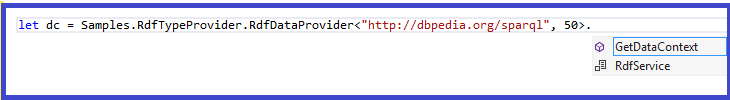
\includegraphics[width=0.99\linewidth]{./figs/getContext.png}
\caption{Methode \texttt{GetDataContext()} to create the data handler}
\label{fig:getdc}
\end{figure}


Accordingly, ``accessing'' the data handler by the dot-operator is an IDE-integrated
access for the navigation and retrieval of data from the external RDF data source.
In particular, using the dot-operator depends from the current \emph{status} of
the data handler. 

\begin{enumerate}
	\item After the instantiation of the data handler, it refers just
	       to the RDF data source, e.g., DBpedia. This is represented
	   by a root type (also called service type) \texttt{http://dbpedia.org}.
		  When pressing the dot, we get a list of all  classes of the data source.
			This is illustrated in Fig.~\ref{fig:showClass}.
			\begin{figure}[h]
				\centering
			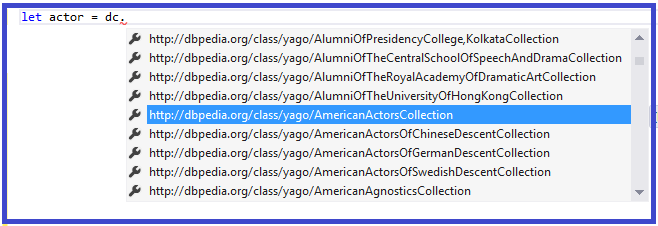
\includegraphics[width=0.99\linewidth]{./figs/getClass.png}
			\caption{Use dot-operator direclty on the data handler}
			\label{fig:showClass}
			\end{figure}
	\item After selecting one of the classes, the status of the data handler refers to this class.
	    For instance, if the developer selects the RDF class ``Actor'' (from the list of classes shown by the data handler),
			the current status of the data handler is an ``Actor'' RDF class.
			% In the program, 			this status is represented by the path \texttt{<http://dbpedia.org/>.<http://dbpedia.org/ontology/Actor>}.
			At this point in time, the type for Actor is not created, only the status of
			the data handler refers to a certain RDF class,e e.g., to ``Actor''.
			
			
  \item When the status of the data handler is a particular class,
		the dot-operator will list all properties of the class and a collection,
		called ``Individuals'', that contains all individuals of this class.
		 \begin{itemize}
			 \item When one of these properties is selected, the status of the data handler is this
			   particular selected property. For instance, for Actor, we can select the
				  property ``\texttt{subClassOf}''. At this point, we are still
						exploring the data source by extending the data handler. Accordingly,
						the type of the class with this property does not exist yet.
						Using the dot-operator on this property, the programmer gets a list of classes
					 that are the super-classes of the domain-class. For instance, the class ``Artist''.
					 When one class of this list is selcted, the status of the data handler is,
					 like in the second case, a certain RDF class (e.g., ``Artist'').
					 % The exploration is shown in Fig.~\ref{fig:showProp}.
			\begin{figure}[h]
				\centering
			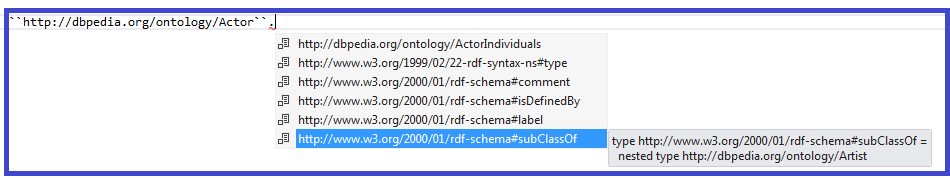
\includegraphics[width=0.99\linewidth]{./figs/getProp.png}
			\caption{Use dot-operator for a class to get properties}
			\label{fig:showProp}
			\end{figure}
					
				
					
				\item When the collection of individuals is selected, the developer gets
					a list of individuals. If one is selected, e.g., ``Bruce Lee'', the
					status of the data handler is the current individual, as examplified in Fig.~\ref{fig:showInd}.
			   \begin{figure}[h]
				 \centering
			   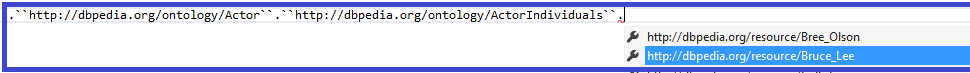
\includegraphics[width=0.99\linewidth]{./figs/getInd.png}
			     \caption{Use dot-operator for a class to get individuals}
		   	\label{fig:showInd}
		   	\end{figure}
					
					
					When using the dot-operator for an individual state,
					 e.g., for ``Bruce Lee'', the developer can see a list of properties,
					but now these are all properties of this particual individual.
		 \end{itemize}
\end{enumerate}


\subsection{Type Definitions}

If the exploration with the data handler is finished the type of the current state of
the data handler is created. An exploration is finished if no further dot operator is
applied and instead the programmer presses \texttt{return}.

The type bridge has a twofold contribution to the programming
environment that is using the bridge. First, it provides the signature from
the information space in terms of a name-space, type names, properties and literals.
Second, the concrete data and the structure of types are obtained. For instance, if
a type for an RDF class is created all the properties of this type are obtained from the
data source and accordingly incorporated in the type definition. An essential aspect is that types are created \emph{on-demand},
i.e., lazily, only if the information is required in the host program then the corresponding type is created. 
Thus, in theory the data source can be very large or even infinite.

Types that are generated by the type bridge are treated as built-in types of the programming language.
Accordingly, the usual type operations can be applied too, including type casts and type inference.


%%%%%%%%%%%%%%%%%%%%%%%%%%%%%%%%%%%%%%%%%%%%%%%%%%%%%%%%%%%%%%%
\section{Scalability Assessment and Implementation}
\label{sec:eval}
%%%%%%%%%%%%%%%%%%%%%%%%%%%%%%%%%%%%%%%%%%%%%%%%%%%%%%%%%%%%%%%

The type bridge is implemented in \fs\footnote{The \fs Software Foundation: \url{http://fsharp.org/}}. It can be used as a library (dll-file) within \fs. 
The type bridge has been tested with several data sources like bio2rdf and DBpedia as the largest data source.
The implementation is scalable with such large data sources. When exploring the data
source using the data handler with the dot-operator, the list of suggestions (as described in Sect.~\ref{sec:usage:retrieval})
is shown to the programmer in less than a second.

The source code, the compiled library and additional descriptions
and explanations with illustrating examples can be found at our project Web site\footnote{RDF Type Bridge: \url{https://github.com/groener/RDFTypeBridge}}.
 
%%%%%%%%%%%%%%%%%%%%%%%%%%%%%%%%%%%%%%%%%%%%%%%%%%%%%%%%%%%%%%%%
\section{Related Work}
\label{sec:rw}
%%%%%%%%%%%%%%%%%%%%%%%%%%%%%%%%%%%%%%%%%%%%%%%%%%%%%%%%%%%%%

% navigation and source exploration
Related work can be distinguished into two groups: the exploration of data sources (data access)
and the integration or mapping of RDF data into programming environments or program code.

The exploration and visualization of data sources 
allow users without SPARQL experiences an easy access to information from linked data sources.
Systems like tFacet~\cite{tFacet}, Facet~\cite{DBLP:conf/semweb/HildebrandOH06} and gFacet~\cite{heim2008gfacet}
offer faceted exploration of linked data sources. gFacet provides a graph facet for browsing
and  fFacet provides a tree view.
The  visualizing parts of a data source in combination with navigation is studied in~\cite{DBLP:conf/iv/DokulilK08}.
However, in this work the focus is clearly on the visualization part.
Compared to our type bridge, none of these approaches consider the integration and typing.

OData\footnote{OData (Open Data Protocol): \url{http://www.odata.org/}}  is a protocol that aims at querying external data via a RESTful service.
OData contains a data model, which is base on an ER model,
and accordingly, the protocol describes types and data.
Mappings from OData applications to SPARQL endpoints
are implemented in the ODATA SPARQL project\footnote{OData SPARQL: \url{https://github.com/BrightstarDB/odata-sparql}}.

% typing
Several work studies the mapping between RDF data / RDF triples of program elements.
In~\cite{oren2008}, mapping principles for RDF triples to objects in object-oriented programming languages are presented.
This work also includes language extensions for the integration.
In \cite{PaarV11}, an extension of the object-oriented language C\# is presented.
The approach offers features to order to represent OWL constructs in C\#.
The typing is similar to our type creation.
The specified types are also created at compile time
and are integrated into the type system of C\#. 
However, the developer must know the structure (schema) of the ontology in order
to define the corresponding types in an OWL-like manner. In contrast, our type bridge
can be used for arbitrary RDF data sources due to the exploration support by using the data handler.

Persistence layers offer a kind of access interface from programs to ontologies.
\`{A}gogo~\cite{AGOGO} is a model-driven approach that offers a development environment
to build mappings between program code and OWL ontologies, and to automatically generate 
an API to access the ontology.
OntoMDE~\cite{conf/esws/ScheglmannSS12} is also model driven approach to generate ontology APIs.
However, both approaches are suited for accessing and integrating a particular known ontology.
Besides this, there is no support of powerful on demand typing and IDE development support
as in our RDF type bridge.


Basic mapping principles are applied
in code generation, in which RDF data are mapped to programming structures.
This is implemented in RDFReactor~\cite{rdfreactor-iswc2005-poster} and Jena~\cite{carroll2004jena}.


In other application domains, integration and typing is studied in different dimensions. 
 In~\cite{GilM08}, structural typing, as known from some functional languages, for Java is presented. 
The principle is comparable to our rules for type definition specifications.
The same holds for the specifications for strongly typed heterogeneous collections in~\cite{BrachaL92,KiselyovLS04}.
These techniques do not allow for the exploration of properties in data sources, as it is needed
for unknown RDF sources.

Tipola~\cite{DBLP:conf/semweb/GangemiNPDMC12} is an algorithm and tool for typing DBpedia entities. The types are obtained by natural language definitions
from Wikipedia in addition with techniques like word sense disambiguation based on WordNet. This seems feasible
for entities where natural languages are available, while our typing approach directly reflects the ontological structure
of the RDF data source in the type system.

%%%%%%%%%%%%%%%%%%%%%%%%%%%%%%%%%%%%%%%%%%%%%%%
\section{Conclusion}
\label{sec:conclusion}

The key investigation of this paper was the integration of RDF data sources
into statically typed programs. These statically programs offer great benefits for
the developer during the program design, e.g., by interactive type checking, type suggestion
and auto-completion. At run-time, statically programs prevent errors and exceptions
that are caused by incompatible types. In the realm of data programming, first attempts
already studied the integration of well-known schematized data sources into statically
typed programs. In this paper, we go one step further and apply similar principles for
RDF data sources where schema information is often missing, incomplete or
the used vocabulary is unknown to the programmer. To remedy this,
we use a data handler to interactively retrieve data from the RDF data source
and integrate the retrieved data into the static type system.
These types, which are provided by the RDF type bridge, are treated
in the programming environment like other built-in types.

As a next step, we plan to extend the type bridge to other more complex representations
like the Web ontology language (OWL). For this purpose, a variety additional constructs
must be considered in the source exploration, but also in the way how types can be specified.

%\subsection{LINQ Query Expressions}
%
%LINQ (language-integrated query) is a set of technologies of query capabilities directly in .NET languages.
%LINQ can transform data from any LINQ enabled data source, like an SQL database, into a .NET program.
%LINQ queries consists of three clauses: (i)~\textsf{from} (specifies the data source)
%(ii)~\textsf{where} (applies filters) and (iii)~\textsf{select} (specifies the type of return element).
%For instance:
%\begin{lstlisting}
%var evenNumQuery = 
     %from num in numbers} 
     %where (num % 2) == 0
     %select num;
%\end{lstlisting}
		%
%LINQ is a standard query language for traversal, filter and projection.
%LINQ is primarily defined for collections and .NET arrays.
%
%
%LINQ seems to be rather simple to extract data from data sources, e.g., given a list of records
%a LINQ query can specify which (parts of) records will be retrieved and what is the condition.
%For instance, the \textbf{data source} can be an array.  Then, the \textbf{query} specifies which information to retrieve from teh data source.
%
%
%
%Linq2Rdf is a semantic Web framework for .NET. It supports the integration of SPARQL queries in \fs programs.
%\url{http://www.hookedonlinq.com/LINQTORDF.ashx}
%
%
%SPARQL query: get all RDF classes: \\
%\begin{lstlisting}
%SELECT DISTINCT ?t WHERE { ?_s rdf:type ?t } LIMIT 100
%\end{lstlisting}
%

%\begin{lstlisting}
%from character in Characters
%where character.Episodes > 120
%select character;
%\end{lstlisting}


%%%%%%%%%%%%%%%%%%%%%%%%%%%%%%%%%%%%%%%%%%%%%%%%%%%%%%%%%%%%%%%%%%%%%%%%%%%%%%%%%
%\section{Discussions Regarding the  Implementation}
%
%%%%%%%%%%%%%%%%%%%%%%%%%%%%%%%%%%%%%%%%%%%%%%%%%%%%%%%%%%%%%%%%%%%%%%%%%%%%%%%%%
%
%\paragraph{Navigation on Individual level}
%
%- if we are at individual level, we only want to navigate on the properties of a particular individual (not on properties of other individuals)
%
%- how are we doing at the class level (problem: in dbpedia we have only four properties defined at the class level --- and this are always the same)
   %+ is the current sampling a meaningful approach?
 %
%%%%%%%%%%%%%%%%%%%%%%%%%%%%%%%%%%%%%%%%%%%%%%%%%%%%%%%%%%%%%%%%%%%%%%%%%%%%%%%%%%%%%%%%%%%%%%%%%%%%%%%%%%%%%%%%%%%%%%

\bibliographystyle{splncs}
\bibliography{references}



\end{document}
